\section{Prosedur Algoritma ElGamal}
\label{sec:prosedur-elgamal}

Sistem ElGamal tersusun dari tiga tahap yang berurutan: pembangkitan pasangan
kunci, enkripsi, dan dekripsi. Ketiganya memakai operasi yang sama, yaitu
perpangkatkan modular, sehingga seluruh sistem hanya memerlukan satu perkakas
aritmetika. Yang membedakan ketiga tahap itu adalah besaran mana yang
diperlakukan sebagai rahasia dan besaran mana yang boleh diketahui umum.

\subsection{Properti dan Kerahasiaan Parameter}

Sebelum menelusuri ketiga tahap itu, ada baiknya seluruh besaran yang terlibat
didaftar lebih dahulu beserta status kerahasiaannya. Daftar itu diperlihatkan
pada Tabel~\ref{tab:parameter-elgamal}.

\begin{table}[htbp]
    \centering
    \begin{tabular}{@{}l l c@{}}
    \toprule
    \textbf{Besaran} & \textbf{Arti} & \textbf{Rahasia?} \\
    \midrule
    $p$          & bilangan prima besar                        & tidak \\
    $g$          & akar primitif dari $p$ dengan $g < p$       & tidak \\
    $x$          & kunci privat, $2 \le x \le p-2$             & \textbf{ya} \\
    $y$          & kunci publik, $y = g^{x} \bmod p$           & tidak \\
    $m$          & plainteks, $0 \le m \le p-1$                & \textbf{ya} \\
    $k$          & kunci efemeral, $1 \le k \le p-2$           & \textbf{ya} \\
    $a, b$       & cipherteks, $a = g^{k} \bmod p$ dan
                   $b = y^{k} m \bmod p$                        & tidak \\
    \bottomrule
    \end{tabular}
    \caption{Besaran pada algoritma ElGamal dan status kerahasiaannya. Pasangan
    $(y, g, p)$ boleh disiarkan; yang harus dijaga adalah $x$, $m$, dan yang
    paling mudah terlupakan, yaitu kunci efemeral $k$}
    \label{tab:parameter-elgamal}
\end{table}

Baris terakhir tabel itu mengandung pasangan $(a, b)$ yang keduanya boleh
dibaca siapa pun. Inilah yang membedakan ElGamal dari kriptografi
kunci-simetri: seluruh bahan yang melewati saluran bersifat terbuka, dan
keamanannya semata-mata bergantung pada kenyataan bahwa $x$ tidak dapat
dihitung dari $y$.

Perlu ditegaskan bahwa baris $k$ bukan sekadar pelengkap. Kunci efemeral $k$
dibangkitkan pengirim, dipakai sekali, lalu dibuang. Ia harus dirahasiakan
sama ketatnya dengan kunci privat, sebab sebagaimana diperlihatkan pada
Subbagian~\ref{subsec:k-ulang}, penggunaannya yang berulang dapat membuka
seluruh plainteks tanpa pernah menyentuh persoalan logaritma diskret.

\subsection{Pembangkitan Pasangan Kunci}
\label{subsec:kunci-elgamal}

Untuk menciptakan pasangan kunci, pemilik kunci melakukan langkah-langkah
berikut.

\begin{enumerate}
    \item Pilih bilangan prima besar $p$. Nilai ini boleh dipakai bersama oleh
          sekelompok pengguna dan tidak perlu dirahasiakan.
    \item Pilih bilangan acak $g$ dengan $g < p$ yang merupakan akar primitif
          dari $p$.
    \item Pilih bilangan bulat acak $x$ sebagai kunci privat, dengan syarat
          $2 \le x \le p-2$.
    \item Hitung kunci publik $y$ dengan rumus
    \begin{equation}
    y = g^{x} \bmod p .
    \label{eq:elgamal-kunci}
    \end{equation}
\end{enumerate}

Hasil dari keempat langkah itu adalah kunci publik berupa tripel
$(y, g, p)$ dan kunci privat berupa pasangan $(x, p)$. Kunci publik disiarkan,
sedangkan $x$ tidak pernah meninggalkan pemiliknya.

Perhatikan batas $2 \le x \le p-2$ pada langkah 3. Kedua ujung selang itu
dikecualikan bukan tanpa alasan. Bila $x = 1$, maka $y = g^{1} = g$, sehingga
kunci publiknya sama persis dengan bilangan yang sudah disiarkan pada
langkah 2; penyerang tidak perlu menghitung apa pun. Bila $x = p - 1$, maka
$y = g^{p-1} \equiv 1 \pmod{p}$ menurut Teorema Kecil Fermat, sehingga kunci
publiknya bernilai tetap $1$ untuk setiap modulus. Kedua nilai itu karena itu
tidak memberi kerahasiaan apa pun, dan selang $2 \le x \le p-2$ menutup
keduanya sekaligus.

Yang perlu dicatat, modulus $p$ muncul pada kunci privat maupun kunci publik.
Kenyataan itu wajar: $p$ memang tidak rahasia, dan menyebutkannya pada kedua
kunci hanya menegaskan bahwa keduanya harus bekerja pada modulus yang sama.

\subsection{Proses Enkripsi}

Misalkan pengirim ingin menyampaikan pesan $m$ kepada pemilik kunci publik
$(y, g, p)$. Langkah-langkahnya adalah sebagai berikut.

\begin{enumerate}
    \item Lakukan \textit{preprocessing}. Bila plainteks berukuran besar, pecah
          plainteks menjadi blok-blok $m_{1}, m_{2}, \dots$ dengan syarat setiap
          blok memenuhi $0 \le m_{i} \le p-1$.
    \item Pilih bilangan acak $k$ sebagai kunci efemeral, dengan $1 \le k \le p-2$.
    \item Untuk setiap blok $m$, hitung pasangan cipherteks
    \begin{align}
    a &= g^{k} \bmod p , \label{eq:elgamal-a} \\
    b &= y^{k} \cdot m \bmod p . \label{eq:elgamal-b}
    \end{align}
\end{enumerate}

Pasangan $(a, b)$ adalah cipherteks untuk blok pesan $m$. Karena setiap blok
menghasilkan dua bilangan, ukuran cipherteks menjadi dua kali ukuran
plainteksnya. Sifat ini disebut \textbf{ekspansi cipherteks} dan dibahas lebih
lanjut pada Subbagian~\ref{subsec:ekspansi-elgamal}.

Syarat $0 \le m_{i} \le p-1$ pada langkah 1 bukan sekadar batas teknis.
Perkalian pada Persamaan~\eqref{eq:elgamal-b} dilakukan modulo $p$, sehingga
dua plainteks yang berbeda $p$ satuan akan menghasilkan cipherteks yang sama
persis. Agar pemulihan pesan bersifat satu-ke-satu, setiap blok harus lebih
kecil daripada modulus --- alasan yang sama dengan pembatasan panjang blok
pada RSA di Bab~\ref{chap:rsa}.

Perhatikan pula bahwa pada Persamaan~\eqref{eq:elgamal-a} nilai $a$ hanya
bergantung pada $g$ dan $k$, tidak pada pesannya. Bagi pengirim yang harus
mengirim pesan panjang, kenyataan itu tampak seperti pemborosan: nilai $a$
dihitung ulang untuk setiap blok padahal rumusnya tidak berubah. Namun justru
itulah yang tidak boleh dilakukan, sebab memakai kembali $k$ yang sama untuk
dua blok berbeda akan membuka keduanya sekaligus, sebagaimana ditunjukkan pada
Subbagian~\ref{subsec:k-ulang}. Kunci efemeral harus dibangkitkan baru untuk
setiap blok.

\subsection{Proses Dekripsi}

Penerima memakai kunci privat $x$ untuk mengembalikan pesan $m$ dari pasangan
$(a, b)$. Langkah pertamanya adalah menghitung invers dari $a^{x}$ modulo $p$:
\begin{equation}
\left(a^{x}\right)^{-1} \equiv a^{\,p-1-x} \pmod{p} .
\label{eq:elgamal-invers}
\end{equation}
Langkah kedua adalah mengalikan cipherteks $b$ dengan invers tersebut:
\begin{equation}
m = b \cdot \left(a^{x}\right)^{-1} \bmod p .
\label{eq:elgamal-dekripsi}
\end{equation}

Mengapa invers pada Persamaan~\eqref{eq:elgamal-invers} dapat dihitung dengan
cara semudah itu? Menurut Teorema Kecil Fermat, $a^{p-1} \equiv 1 \pmod{p}$
selama $a$ tidak habis dibagi $p$. Karena itu
\[ a^{x} \cdot a^{\,p-1-x} = a^{\,p-1} \equiv 1 \pmod{p} , \]
yang berarti $a^{\,p-1-x}$ memang invers perkalian dari $a^{x}$ modulo $p$.
Cara ini menghindari algoritma Euclidean diperluas yang dipakai pada
Bab~\ref{chap:rsa}: cukup satu perpangkatkan modular, sama seperti langkah
lainnya.

\subsection{Mengapa Dekripsi Berhasil}
\label{subsec:bukti-elgamal}

Rumus dekripsi pada Persamaan~\eqref{eq:elgamal-dekripsi} baru dapat dipercaya
setelah dibuktikan bahwa hasilnya memang plainteks semula. Bukti itu disusun
dari ketiga persamaan yang sudah ada.

Dari Persamaan~\eqref{eq:elgamal-a} diperoleh $g^{k} \equiv a \pmod{p}$.
Pangkatkan kedua ruas dengan $x$, maka
$g^{xk} \equiv a^{x} \pmod{p}$. Sementara itu dari
Persamaan~\eqref{eq:elgamal-kunci} diperoleh $g^{x} \equiv y \pmod{p}$,
sehingga $y^{k} \equiv g^{xk} \pmod{p}$. Substitusikan kedua hasil itu ke dalam
Persamaan~\eqref{eq:elgamal-b}:

\begin{equation}
\begin{split}
\frac{b}{a^{x}} &\equiv \frac{y^{k} m}{a^{x}} \pmod{p} \\
                &\equiv \frac{g^{xk} m}{g^{xk}} \pmod{p} \\
                &\equiv m \pmod{p} .
\end{split}
\label{eq:elgamal-bukti}
\end{equation}

Rantai kesamaan pada Persamaan~\eqref{eq:elgamal-bukti} memperlihatkan bahwa
faktor $g^{xk}$ muncul pada pembilang maupun penyebut, sehingga saling
meniadakan. Yang tersisa hanyalah $m$. Dengan kata lain, plainteks dapat
diungkap kembali dari cipherteks $(a, b)$ semata, tanpa memerlukan keterangan
tambahan apa pun dari pengirim.

Perhatikan bahwa pembuktian itu sama sekali tidak menyentuh persoalan
logaritma diskret. Dekripsi berhasil karena Bob memegang $x$, dan $x$ itulah
yang memungkinkan ia membentuk $g^{xk}$ dari $a = g^{k}$. Seorang penyerang
yang hanya menyadap $a$ tidak dapat melakukan langkah yang sama, sebab ia tidak
dapat memisahkan $k$ dari $g^{k}$.

% Alur algoritma ElGamal: pembangkitan kunci, enkripsi dengan kunci acak k,
% dekripsi memakai kunci privat x.
% Dirujuk dari section-03.tex dengan % Alur algoritma ElGamal: pembangkitan kunci, enkripsi dengan kunci acak k,
% dekripsi memakai kunci privat x.
% Dirujuk dari section-03.tex dengan % Alur algoritma ElGamal: pembangkitan kunci, enkripsi dengan kunci acak k,
% dekripsi memakai kunci privat x.
% Dirujuk dari section-03.tex dengan \input{figures/alur-elgamal}.
\begin{figure}[htbp]
    \centering
    \begin{tikzpicture}[
        kotak/.style={draw, rounded corners, align=center, font=\small, inner sep=5pt},
        panah/.style={-{Latex[length=2.4mm]}, thick},
        kunci/.style={-{Latex[length=2.4mm]}, thick, dashed, gray!75},
    ]
        \node[kotak, fill=gray!10, minimum width=8.4cm] (gen) at (2.6,0)
            {Pembangkitan kunci: pilih prima $p$ dan akar primitif $g$;\\
             pilih kunci privat $x$ lalu hitung $y = g^{x} \bmod p$};
        \node[kotak, fill=blue!6, minimum width=3.2cm] (pub)  at (0.4,-1.8) {Kunci publik $(y, g, p)$};
        \node[kotak, fill=red!6,  minimum width=3.2cm] (priv) at (5.6,-1.8) {Kunci privat $x$};

        \draw[panah] (gen.south) -- ++(0,-0.4) -| (pub.north);
        \draw[panah] (gen.south) -- ++(0,-0.4) -| (priv.north);

        \node[kotak, fill=green!10,  minimum width=2.4cm] (m)   at (-2.8,-4.0) {Pesan $m$};
        \node[kotak, fill=orange!12, minimum width=3.6cm] (enc) at (0.5,-4.0)
            {pilih $k$ acak;\\ $a = g^{k} \bmod p$;\\ $b = y^{k} m \bmod p$};
        \node[kotak, fill=green!10,  minimum width=1.4cm] (c)   at (3.3,-4.0)  {$(a, b)$};
        \node[kotak, fill=orange!12, minimum width=3.4cm] (dec) at (6.2,-4.0)
            {$m = b \cdot (a^{x})^{-1}$\\ $\bmod p$};
        \node[kotak, fill=green!10,  minimum width=2.4cm] (m2)  at (9.4,-4.0)  {Pesan $m$};

        \draw[kunci] (pub.south)  -- (enc.north);
        \draw[kunci] (priv.south) -- (dec.north);

        \draw[panah] (m) -- (enc);
        \draw[panah] (enc) -- (c);
        \draw[panah] (c) -- (dec);
        \draw[panah] (dec) -- (m2);
    \end{tikzpicture}
    \caption{Alur algoritma ElGamal: cipherteks berupa pasangan $(a, b)$ dan berubah setiap kali karena kunci acak $k$}
    \label{fig:alur-elgamal}
\end{figure}
.
\begin{figure}[htbp]
    \centering
    \begin{tikzpicture}[
        kotak/.style={draw, rounded corners, align=center, font=\small, inner sep=5pt},
        panah/.style={-{Latex[length=2.4mm]}, thick},
        kunci/.style={-{Latex[length=2.4mm]}, thick, dashed, gray!75},
    ]
        \node[kotak, fill=gray!10, minimum width=8.4cm] (gen) at (2.6,0)
            {Pembangkitan kunci: pilih prima $p$ dan akar primitif $g$;\\
             pilih kunci privat $x$ lalu hitung $y = g^{x} \bmod p$};
        \node[kotak, fill=blue!6, minimum width=3.2cm] (pub)  at (0.4,-1.8) {Kunci publik $(y, g, p)$};
        \node[kotak, fill=red!6,  minimum width=3.2cm] (priv) at (5.6,-1.8) {Kunci privat $x$};

        \draw[panah] (gen.south) -- ++(0,-0.4) -| (pub.north);
        \draw[panah] (gen.south) -- ++(0,-0.4) -| (priv.north);

        \node[kotak, fill=green!10,  minimum width=2.4cm] (m)   at (-2.8,-4.0) {Pesan $m$};
        \node[kotak, fill=orange!12, minimum width=3.6cm] (enc) at (0.5,-4.0)
            {pilih $k$ acak;\\ $a = g^{k} \bmod p$;\\ $b = y^{k} m \bmod p$};
        \node[kotak, fill=green!10,  minimum width=1.4cm] (c)   at (3.3,-4.0)  {$(a, b)$};
        \node[kotak, fill=orange!12, minimum width=3.4cm] (dec) at (6.2,-4.0)
            {$m = b \cdot (a^{x})^{-1}$\\ $\bmod p$};
        \node[kotak, fill=green!10,  minimum width=2.4cm] (m2)  at (9.4,-4.0)  {Pesan $m$};

        \draw[kunci] (pub.south)  -- (enc.north);
        \draw[kunci] (priv.south) -- (dec.north);

        \draw[panah] (m) -- (enc);
        \draw[panah] (enc) -- (c);
        \draw[panah] (c) -- (dec);
        \draw[panah] (dec) -- (m2);
    \end{tikzpicture}
    \caption{Alur algoritma ElGamal: cipherteks berupa pasangan $(a, b)$ dan berubah setiap kali karena kunci acak $k$}
    \label{fig:alur-elgamal}
\end{figure}
.
\begin{figure}[htbp]
    \centering
    \begin{tikzpicture}[
        kotak/.style={draw, rounded corners, align=center, font=\small, inner sep=5pt},
        panah/.style={-{Latex[length=2.4mm]}, thick},
        kunci/.style={-{Latex[length=2.4mm]}, thick, dashed, gray!75},
    ]
        \node[kotak, fill=gray!10, minimum width=8.4cm] (gen) at (2.6,0)
            {Pembangkitan kunci: pilih prima $p$ dan akar primitif $g$;\\
             pilih kunci privat $x$ lalu hitung $y = g^{x} \bmod p$};
        \node[kotak, fill=blue!6, minimum width=3.2cm] (pub)  at (0.4,-1.8) {Kunci publik $(y, g, p)$};
        \node[kotak, fill=red!6,  minimum width=3.2cm] (priv) at (5.6,-1.8) {Kunci privat $x$};

        \draw[panah] (gen.south) -- ++(0,-0.4) -| (pub.north);
        \draw[panah] (gen.south) -- ++(0,-0.4) -| (priv.north);

        \node[kotak, fill=green!10,  minimum width=2.4cm] (m)   at (-2.8,-4.0) {Pesan $m$};
        \node[kotak, fill=orange!12, minimum width=3.6cm] (enc) at (0.5,-4.0)
            {pilih $k$ acak;\\ $a = g^{k} \bmod p$;\\ $b = y^{k} m \bmod p$};
        \node[kotak, fill=green!10,  minimum width=1.4cm] (c)   at (3.3,-4.0)  {$(a, b)$};
        \node[kotak, fill=orange!12, minimum width=3.4cm] (dec) at (6.2,-4.0)
            {$m = b \cdot (a^{x})^{-1}$\\ $\bmod p$};
        \node[kotak, fill=green!10,  minimum width=2.4cm] (m2)  at (9.4,-4.0)  {Pesan $m$};

        \draw[kunci] (pub.south)  -- (enc.north);
        \draw[kunci] (priv.south) -- (dec.north);

        \draw[panah] (m) -- (enc);
        \draw[panah] (enc) -- (c);
        \draw[panah] (c) -- (dec);
        \draw[panah] (dec) -- (m2);
    \end{tikzpicture}
    \caption{Alur algoritma ElGamal: cipherteks berupa pasangan $(a, b)$ dan berubah setiap kali karena kunci acak $k$}
    \label{fig:alur-elgamal}
\end{figure}


\begin{figure}[htbp]
    \centering
    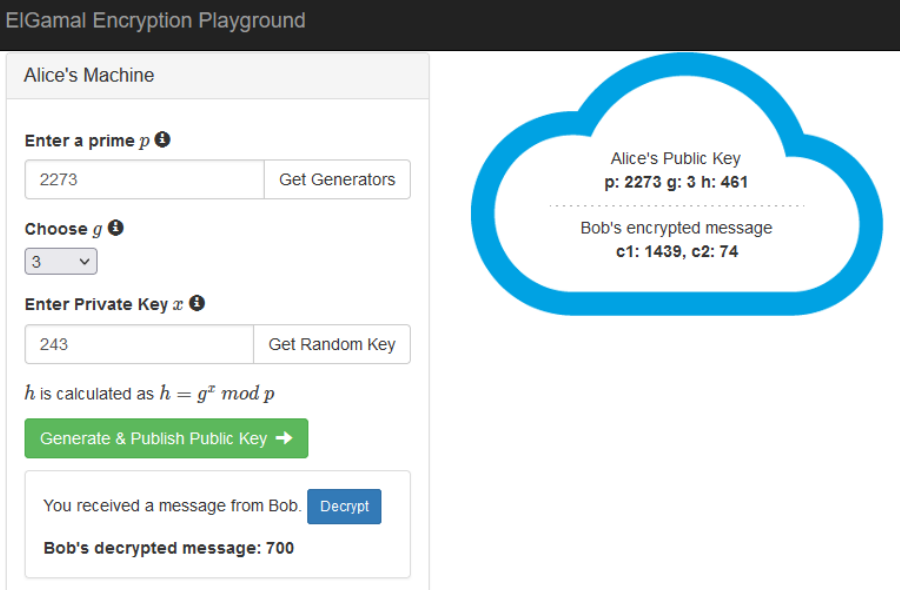
\includegraphics[width=0.78\linewidth, height=0.72\textheight, keepaspectratio]{figures/simulasi-enkripsi-elgamal.png}
    \caption{Contoh enkripsi dan dekripsi ElGamal pada sebuah simulasi daring:
    dengan $p = 2273$, $g = 3$, $x = 243$, dan $y = 461$, pesan $m = 700$
    dienkripsi menjadi pasangan $(c_{1}, c_{2}) = (1439, 74)$ lalu dipulihkan
    kembali. Perkakas itu menamai kunci publik dengan $h$, bukan $y$}
    \label{fig:simulasi-enkripsi-elgamal}
    \sumber{Munir, \textit{IF4020 Kriptografi}, ITB.}
\end{figure}
